\documentclass[border=4pt]{standalone}
\usepackage{fontspec}
\setmainfont{Times New Roman}
\setmonofont{Consolas}
\usepackage{tikz}
\usetikzlibrary{arrows.meta,positioning,shapes.geometric,calc}
\definecolor{tutorteal}{HTML}{087F7A}
\definecolor{tutorlight}{HTML}{EDF7F5}
\definecolor{tutorink}{HTML}{20323C}
\newcommand{\code}[1]{\texttt{\detokenize{#1}}}
\tikzset{box/.style={draw=tutorteal,rounded corners=2pt,fill=tutorlight,
 align=center,minimum height=10mm,text width=35mm,font=\small,inner sep=5pt},
 decision/.style={diamond,aspect=2.0,draw=tutorteal,fill=white,align=center,
 text width=23mm,font=\small,inner sep=1pt},
 flow/.style={-{Latex[length=2mm]},thick,draw=tutorink},
 optional/.style={flow,dashed}}
\begin{document}
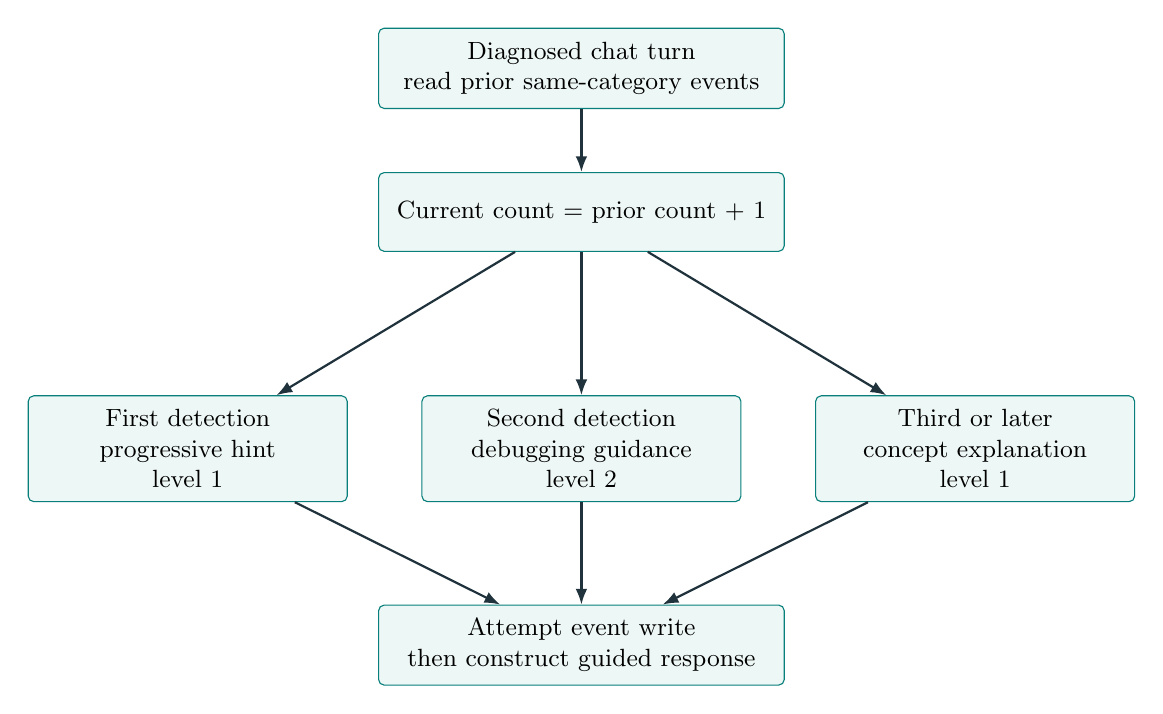
\begin{tikzpicture}[node distance=8mm and 8mm]
\node[box,text width=48mm] (history) {Diagnosed chat turn\\read prior same-category events};
\node[box,text width=48mm,below=of history] (n) {Current count = prior count + 1};
\node[box,text width=37mm] (first) at ($(n.south)+(-50mm,-25mm)$) {First detection\\progressive hint\\level 1};
\node[box,text width=37mm] (second) at ($(n.south)+(0,-25mm)$) {Second detection\\debugging guidance\\level 2};
\node[box,text width=37mm] (third) at ($(n.south)+(50mm,-25mm)$) {Third or later\\concept explanation\\level 1};
\node[box,text width=48mm,below=13mm of second] (record) {Attempt event write\\then construct guided response};
\draw[flow] (history)--(n);
\draw[flow] (n)--(first);
\draw[flow] (n)--(second);
\draw[flow] (n)--(third);
\draw[flow] (first)--(record);
\draw[flow] (second)--(record);
\draw[flow] (third)--(record);
\end{tikzpicture}
\end{document}
